\section{Virksomhedsprofil}

Banken �bnede i januar 2001, som repr�sentationskontor for den islandske Kaupthing Bank. Her var banken 75\% ejet af Kaupthing og 25\% af F�roya Sparikassi. F�roya Sparikassi er F�r�ernes f�rste og st�rste pengeinstitut og blev stiftet i 1832. 1. januar 2005 opk�bte F�roya Sparikassi Kaupthings del af selskabet og det blev navngivet EIK Bank Danmark A/S. EIK er det f�r�ske ord for det solide gamle egetr�, der i mange �r har v�ret f�lles logo for de danske sparekasser.

Siden da har banken v�ret i kraftig v�kst, hvilket afspejles i halv\-�rs\-re\-sul\-ta\-tet for EIK Bank der steg fra 7,3 mio. kr. f�rste halv�r 2004 til 15,2 mio.kr. f�rste halv�r 2005. Balancen steg med 43\% til 1,5 mia. kr. fra ultimo juni 2004 til ultimo juni 2005. Banken er medlem af K�benhavns Fondsb�rs og leverer tjenesteydelser indenfor private banking, investerings\-r�dgivning, pantebrevshandel samt ejendoms- og projektfinansiering. R�d\-giverne i banken har alle direkte kontakt til b�rsmarkedet. Banken har i dag 40 ansatte i dens ejendom p� N�rre Farimagsgade 15 i K�benhavn.

Bankens m�l er langsigtede kunde\-relationer, i form af uvildig finansiel r�d\-givning.

I forbindelse med brugernes PC-kundskaber, kan medarbejderne generelt betegnes som brugere p� normalt nivaeu.

\begin{center}
\begin{figure}[h]
	\centering
		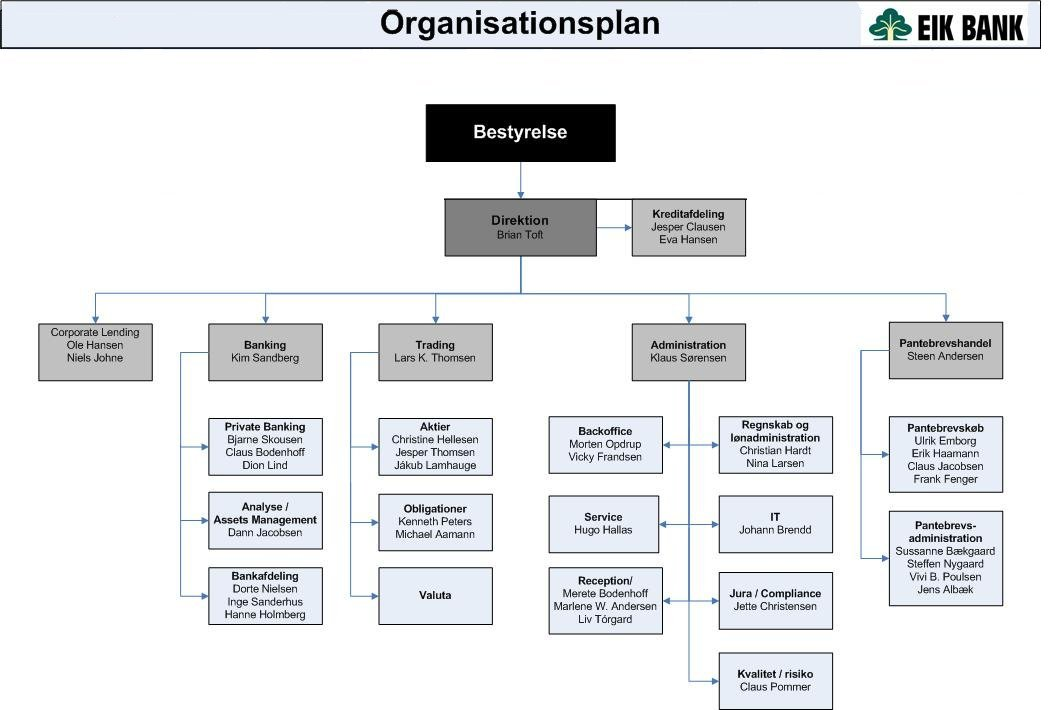
\includegraphics[scale=1.1, width=1.0\textwidth]{Billeder/Organisationsplan.jpg}
	\caption{Organisationsplan}
	\label{Organisationsplan}
\end{figure}
\end{center}



